\chapter{Data description}

\section{Dataset description}
%Descrizione del dataset (parziale), vincoli: non tutti i farmaci etici passano dal medico di base (ricette rosse, medici ospedalieri), mentre farmacie/anagrafe tributarie sono completi
%Non esiste una relazione diretta tra prescrizione e acquisto di prodotto
%Non sempre le prescrizioni non sono centrate sul pazienti

% handling sensitive data

\section{Overview of the database}
The database used for analytics contains data on medical histories of patients between \textbf{January 2000} and \textbf{October 2018}. This leads to some observations:
\begin{enumerate}
	\item The year 2018 is present only up to June, so it cannot be used while making time series within years (there is going to be a drop of values due to incompleteness which may lead to wrong conclusions);
	\item A timespan of 20 years is too wide to make consistent analytics;
	\item Early dated records might contain outdated or incomplete information.
\end{enumerate}

Global inferences have been made with the entire dataset, while the need of detailed recent reports leads to the decision of using a limited range of years for prescription pattern changes and patient journey.

The research work has been done on only a part of the original Millewin database, consisting in \textbf{4 tables}. There is information available on \textbf{general practitioners}, \textbf{patients}, \textbf{diagnoses} and \textbf{prescriptions}: each macro-category is included in a separated table, so it's necessary to identify the relationship between fields.

The 4 tables with their sizes are:
\begin{itemize}
	\item \textit{patients}, 1.015.618 tuples; \\
	Basic information about patients, identified by an encrypted UID;
	\item \textit{patients\_doctors}, 1.015.618 tuples; \\
	Extension of \textit{patients} with the same key, containing more detailed information about patient-doctor relationships and linkage with GPs identifiers;
	\item \textit{diagnoses}, 15.460.199 tuples; \\
	Information about diagnoses and relative description;
	\item \textit{prescriptions}, 118.716.403 tuples; \\
	Information about therapies and prescribed medicines.
\end{itemize}

It is noticeable that the number of rows is varying: there are more prescriptions than diagnoses, since the first tend to happen more often.

Each diagnosis and prescription is uniquely distinguished by the triplet {patient, doctor, date}. Dates are at level of timestamp, making each one different from the others (it's improbable to have a diagnosis or prescription for the same patient, by the same doctor and at the same exact moment). 

Analysis is performed using dates in the \textit{YYYY-MM-DD} format, since non-unique data still allows to aggregate results and identify patterns. There are several different prescriptions for the same patient made on the same day.

\section{Description of the tables}
Below is reported a brief description of the 4 tables, along with the main fields used for analytics, statistics and meaning.

\subsection{\textit{patients}}
The table \textit{patients} includes information about patients. To ensure privacy dealing with sensitive data, there are no full names: everything is \textbf{encrypted} as a 22-character string containing letters, numbers and special symbols.

Other relevant fields are:
\begin{itemize}
	\item \textit{date}, date of beginning of the doctor-patient relationship;
	\item \textit{birthdate}, date of birth;
	\item \textit{death}, eventual date of death;
	\item \textit{birth\_municipality}, name (and code) of the birth municipality;
	\item \textit{sex}, birth sex;
	\item \textit{convention}, type of convention with the Italian insurance system.
\end{itemize}

\subsection{\textit{patients\_doctors}}
The table \textit{patients\_doctors} contains information similar to \textit{pazienti}, with additional fields focussing on their relationship with the general practitioners, which are essential to link and analyse data:
\begin{itemize}
	\item \textit{doctor}, \textbf{encrypted} UID of the general practitioner of the patient;
	\item \textit{postcode}, zip-code of the patient (for geographical analysis);
	\item \textit{province}, province of the patient;
	\item \textit{revocation}, eventual date of termination of the doctor-patient relationship (a patient changing GP).
\end{itemize}

All the IDs of the GPs, along with all other data on GPs, are stored in an external table \textit{users} (the research has been made considering a subset of the original DB). The latter does not contain any other information relevant for analysis, since active doctors can be extracted from other tables.

\subsection{\textit{diagnoses}}
The table \textit{diagnoses} comprehends the diagnoses associated to patients and relative GPs. Each diagnosis is defined by its \textbf{ICD-9} code, an international identifier for diseases maintained by the World Health Organization. 

Summary of most important features:
\begin{itemize}
	\item \textit{id}, patient ID from \textit{patients};
	\item \textit{userid}, corresponding to \textit{doctor} in \textit{patient\_doctor} (general practitioner ID);
	\item \textit{date}, date of insertion of the diagnosis in the database;
	\item \textit{last\_update}, timestamp of last edit of the tuple;
	\item \textit{description}, a textual description of the diagnosis;
	\item \textit{IDC9}, code of the diagnosis according to the ICD-9 standards.
\end{itemize}

\subsection{\textit{prescriptions}}
The table \textit{prescriptions} contains the prescribed medicines for each patient. There is no linkage between diagnosis and prescriptions in the database, so additional work is required to detect correlation.

Each prescription is defined by an \textbf{ATC code}, from the Anatomical Therapeutical Chemical classification system maintained by the World Health Organization. Furthermore, there are \textbf{active principle code} and \textbf{authorisation for commerce code}(AIC).

Fields summary:
\begin{itemize}
	\item \textit{id}, patient ID;
	\item \textit{userid}, corresponding to \textit{pa\_medi }in \textit{nos\_002} (general practitioner ID);
	\item \textit{date}, date of insertion of the prescription in the database;
	\item \textit{last\_update}, timestamp of last edit of the tuple;
	\item \textit{AIC}, AIC code (authorisation for commerce);
	\item \textit{description}, textual description of the medicine with dosage;
	\item \textit{pieces}, number of boxes;
	\item \textit{active\_principle}, active principle code;
	\item \textit{ATC}, ATC code;
	\item \textit{euro}, price.
\end{itemize}

\section{ER model}
After identifying the main fields, it is possible to build and include an \textbf{ER model}\cite{draw} to have a better understanding of the tables and their relationships.
\begin{figure}[h]
	\centering
	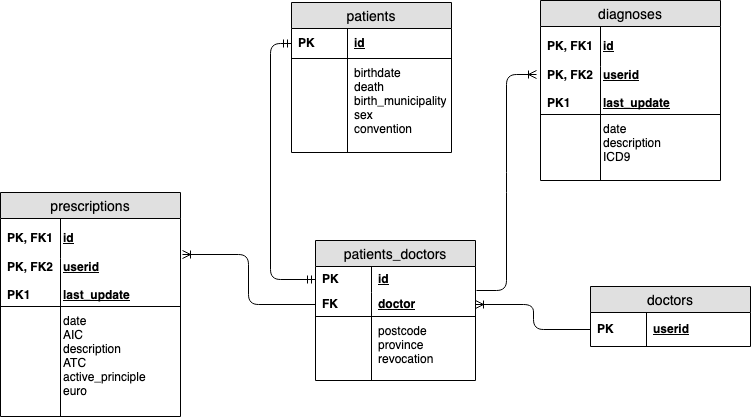
\includegraphics[scale=0.3]{images/er.png} % todo rifare
\end{figure}

\section{Variations through time}
To give a general idea of variations of patients, a snapshot of 2008-2017 is used to show patterns and differences, counting the number of patients having at least one prescription:
%\begin{center}
%	\begin{tabular}{c|c|c|c|c|c|c|c|c|c|c|c}
%		Characteristic & 2008 & 2009 & 2009 & 2010 & 2011 & 2012 & 2013 & 2014 & 2015 & 2016 & 2017 \\
%		Patients number 
%		Age mean
%		Age variance
%		Women \%
%		Men \%
%	\end{tabular}
%\end{center}

An analogue example can be obtained counting the number of diagnoses each year:


